\documentclass[11pt,a4paper]{article}
\usepackage{graphicx,fancyhdr,natbib,subfigure}
\usepackage{epsfig, epsf}
\usepackage{amsmath, cancel, amssymb}
\usepackage{lscape, longtable, caption}
\usepackage{multirow}
\usepackage{dcolumn}% Align table columns on decimal point
\usepackage{bm}% bold math
\usepackage{hyperref,ifthen}
\usepackage{verbatim}
\usepackage{color}
\usepackage[usenames,dvipsnames]{xcolor}
%% http://en.wikibooks.org/wiki/LaTeX/Colors



%%%%%%%%%%%%%%%%%%%%%%%%%%%%%%%%%%%%%%%%%%%
%       define Journal abbreviations      %
%%%%%%%%%%%%%%%%%%%%%%%%%%%%%%%%%%%%%%%%%%%
\def\nat{Nat} \def\apjl{ApJ~Lett.} \def\apj{ApJ}
\def\apjs{ApJS} \def\aj{AJ} \def\mnras{MNRAS}
\def\prd{Phys.~Rev.~D} \def\prl{Phys.~Rev.~Lett.}
\def\plb{Phys.~Lett.~B} \def\jhep{JHEP} \def\nar{NewAR}
\def\npbps{NUC.~Phys.~B~Proc.~Suppl.} \def\prep{Phys.~Rep.}
\def\pasp{PASP} \def\aap{Astron.~\&~Astrophys.} \def\araa{ARA\&A}
\def\pasa{PASA}
\def\jcap{\ref@jnl{J. Cosmology Astropart. Phys.}}%
\def\physrep{Phys.~Rep.}


\newcommand{\preep}[1]{{\tt #1} }

%%%%%%%%%%%%%%%%%%%%%%%%%%%%%%%%%%%%%%%%%%%%%%%%%%%%%
%              define symbols                       %
%%%%%%%%%%%%%%%%%%%%%%%%%%%%%%%%%%%%%%%%%%%%%%%%%%%%%
\def \Mpc {~{\rm Mpc} }
\def \Om {\Omega_0}
\def \Omb {\Omega_{\rm b}}
\def \Omcdm {\Omega_{\rm CDM}}
\def \Omlam {\Omega_{\Lambda}}
\def \Omm {\Omega_{\rm m}}
\def \ho {H_0}
\def \qo {q_0}
\def \lo {\lambda_0}
\def \kms {{\rm ~km~s}^{-1}}
\def \kmsmpc {{\rm ~km~s}^{-1}~{\rm Mpc}^{-1}}
\def \hmpc{~\;h^{-1}~{\rm Mpc}} 
\def \hkpc{\;h^{-1}{\rm kpc}} 
\def \hmpcb{h^{-1}{\rm Mpc}}
\def \dif {{\rm d}}
\def \mlim {m_{\rm l}}
\def \bj {b_{\rm J}}
\def \mb {M_{\rm b_{\rm J}}}
\def \mg {M_{\rm g}}
\def \qso {_{\rm QSO}}
\def \lrg {_{\rm LRG}}
\def \gal {_{\rm gal}}
\def \xibar {\bar{\xi}}
\def \xis{\xi(s)}
\def \xisp{\xi(\sigma, \pi)}
\def \Xisig{\Xi(\sigma)}
\def \xir{\xi(r)}
\def \max {_{\rm max}}
\def \gsim { \lower .75ex \hbox{$\sim$} \llap{\raise .27ex \hbox{$>$}} }
\def \lsim { \lower .75ex \hbox{$\sim$} \llap{\raise .27ex \hbox{$<$}} }
\def \deg {^{\circ}}
%\def \sqdeg {\rm deg^{-2}}
\def \deltac {\delta_{\rm c}}
\def \mmin {M_{\rm min}}
\def \mbh  {M_{\rm BH}}
\def \mdh  {M_{\rm DH}}
\def \msun {M_{\odot}}
\def \z {_{\rm z}}
\def \edd {_{\rm Edd}}
\def \lin {_{\rm lin}}
\def \nonlin {_{\rm non-lin}}
\def \wrms {\langle w_{\rm z}^2\rangle^{1/2}}
\def \dc {\delta_{\rm c}}
\def \wp {w_{p}(\sigma)}
\def \PwrSp {\mathcal{P}(k)}
\def \DelSq {$\Delta^{2}(k)$}
\def \WMAP {{\it WMAP \,}}
\def \cobe {{\it COBE }}
\def \COBE {{\it COBE \;}}
\def \HST  {{\it HST \,\,}}
\def \Spitzer  {{\it Spitzer \,}}
\def \ATLAS {VST-AA$\Omega$ {\it ATLAS} }
\def \BEST   {{\tt best} }
\def \TARGET {{\tt target} }
\def \TQSO   {{\tt TARGET\_QSO}}
\def \HIZ    {{\tt TARGET\_HIZ}}
\def \FIRST  {{\tt TARGET\_FIRST}}
\def \zc {z_{\rm c}}
\def \zcz {z_{\rm c,0}}

\newcommand{\ltsim}{\raisebox{-0.6ex}{$\,\stackrel
        {\raisebox{-.2ex}{$\textstyle <$}}{\sim}\,$}}
\newcommand{\gtsim}{\raisebox{-0.6ex}{$\,\stackrel
        {\raisebox{-.2ex}{$\textstyle >$}}{\sim}\,$}}
\newcommand{\simlt}{\raisebox{-0.6ex}{$\,\stackrel
        {\raisebox{-.2ex}{$\textstyle <$}}{\sim}\,$}}
\newcommand{\simgt}{\raisebox{-0.6ex}{$\,\stackrel
        {\raisebox{-.2ex}{$\textstyle >$}}{\sim}\,$}}

\newcommand{\Msun}{M_\odot}
\newcommand{\Lsun}{L_\odot}
\newcommand{\lsun}{L_\odot}
\newcommand{\Mdot}{\dot M}

\newcommand{\sqdeg}{deg$^{-2}$}
\newcommand{\hi}{H\,{\sc i}\ }
\newcommand{\lya}{Ly$\alpha$\ }
%\newcommand{\lya}{Ly\,$\alpha$\ }
\newcommand{\lyaf}{Ly\,$\alpha$\ forest}
%\newcommand{\eg}{e.g.~}
%\newcommand{\etal}{et~al.~}
\newcommand{\lyb}{Ly$\beta$\ }
\newcommand{\cii}{C\,{\sc ii}\ }
\newcommand{\ciii}{C\,{\sc iii}]\ }
\newcommand{\civ}{C\,{\sc iv}\ }
\newcommand{\SiII}{Si\,{\sc ii}\ }
\newcommand{\SiIV}{Si\,{\sc iv}\ }
\newcommand{\mgii}{Mg\,{\sc ii}\ }
\newcommand{\feii}{Fe\,{\sc ii}\ }
\newcommand{\feiii}{Fe\,{\sc iii}\ }
\newcommand{\caii}{Ca\,{\sc ii}\ }
\newcommand{\halpha}{H\,$\alpha$\ }
\newcommand{\hbeta}{H\,$\beta$\ }
\newcommand{\hgamma}{H\,$\gamma$\ }
\newcommand{\hdelta}{H\,$\delta$\ }
\newcommand{\oi}{[O\,{\sc i}]\ }
\newcommand{\oii}{[O\,{\sc ii}]\ }
\newcommand{\oiii}{[O\,{\sc iii}]\ }
\newcommand{\heii}{He\,{\sc ii}\ }
%\newcommand{\heii}{[He\,{\sc ii}]\ }
\newcommand{\nv}{N\,{\sc v}\ }
\newcommand{\nev}{Ne\,{\sc v}\ }
\newcommand{\neiii}{[Ne\,{\sc iii}]\ }
\newcommand{\alii}{Al\,{\sc ii}\ }
\newcommand{\aliii}{Al\,{\sc iii}\ }
\newcommand{\siiii}{Si\,{\sc iii}]\ }



\begin{document}

\title{Combing the WISE W4 catalogue and the Gaia Data Release 1:
Searching for Infrared bright, optically faint objects across the full
sky.}
 % \author{AUTHOR HERE}
 %\date{\today}
\maketitle

\section*{Preamble}
All the code and plotting packages, and smaller catalogues are
available at \href{https://github.com/d80b2t/WW4C}{{\tt
https://github.com/d80b2t/WW4C}}.  The .tex and PDF file can be found
\href{https://github.com/d80b2t/WW4C/tree/master/LaTeX/GaiaDR1_catalog}{{\tt
here}}.

\noindent
The four `obvious' files that aren't on the GitHub are:: \\
GaiaDR1xWISEw4\_10as\_noDupes\_sorted.csv (1.1G); \\
WISE\_W4\_DecOrdered.dat (1.4GB);\\
WISE\_W4\_cat\_with\_GaiaNull.csv  (2.6GB);\\
WISE\_W4\_cat\_with\_Gaia.csv  (3.2GB).\\



\section{Motivation}
The WISE W4 23$\mu$m band is shallow. Therefore, anything that is detected in
W4, and is {\it not} a Milky Way star, or nearby e.g. dusty spiral
galaxy, is going to be intrinsically very luminous. Furthermore,
objects that are also detected in W4, but are faint/non-detected in
the optical, or in the shorter WISE W1/W2 bands also have very
interesting properties, \citep[e.g.,][]{Assef15, Tsai15, Lonsdale15,
Assef16, Diaz-Santos16, Ricci17, Wu17, Jones17, Farrah17}.  The WISE
W4 band is also crucial in the discovery and characterization of the
``Extremely Red Quasar'' population, using a colour selection of
$r_{\rm AB} − W4_{\rm Vega} >14.0$ \citep{Ross15, Zakamska16,
Hamann17}.

Note, the W4 channel effective wavelength was recalibrated from the
original 22$\mu$m by \citet{Brown14b}.


\section{Matching the Gaia DR1 and WISE W4 catalogs}

    \subsection{WISE}
    The Wide-field Infrared Survey Explorer (WISE) mission description and
    initial on-orbit performance is described in \citet[][]{Wright10}.
    We use the \href{http://wise2.ipac.caltech.edu/docs/release/allwise/expsup/}
    {\tt AllWISE Data Release}. 

    There are 40,939,966 objects, with $>2\sigma$ detections at WISE
    W4 in the AllWISE Catalog. The W4 PSF is 12'', but the centroid
    positions should be good to $\lesssim2''$ (WISE HelpDesk,
    priv. comm.).  Figure~\ref{fig:fig1} shows the sky distribution of
    these 40.9M objects.  The WISE scanning pattern can clearly be 
    \href{http://wise2.ipac.caltech.edu/docs/release/allwise/expsup/sec4_2.html}{{\tt
      seen}}.

    \subsection{Gaia DR1} 
    We use the \href{https://www.cosmos.esa.int/web/gaia/dr1}{{\tt Gaia Data Release 1}}.
    \citep{Gaia16a, Gaia16b}\footnote{I don't know how to fix this citation.}
%    \citep{Prusti16, Brown16}.
    % Gaia Collaboration, Prusti, T., de Bruijne, J. H. J., et al. 2016, A & A, 595, A1
    % Gaia Collaboration, Brown, A. G. A., Vallenari, A., et al. 2016, A & A, 595, A2
    % The Gaia mission Gaia Collaboration, Prusti, T., de Bruijne, J.H.J., et al., 2016a (arXiv)
    % Gaia Data Release 1: Summary of the astrometric, photometric, and survey properties Gaia Collaboration, Brown, A.G.A., Vallenari, A., et al., 2016b (arXiv)
    %% (What about the ten or so other Gaia Data Release 1 papers??!!) 
    %% Gaia Data Release 1: On-orbit performance of the Gaia CCDs at L2 Crowley et al. (arXiv) 
    %% Gaia Data Release 1: Pre-processing and source list creation Fabricius et al. (arXiv)
    %% Gaia Data Release 1: Astrometry: one billion positions, two million proper motions and parallaxes Lindegren et al. (arXiv)
    %% Gaia Data Release 1: The photometric data van Leeuwen et al. (arXiv)
    %% Gaia Data Release 1: Principles of the Photometric Calibration of the G band Carrasco et al. (arXiv)
    %% Gaia Data Release 1: Validation of the Photometry Evans et al. (arXiv)
    %% Gaia Data Release 1: Catalogue validation Arenou et al. (arXiv)
    %% Gaia Data Release 1: The reference frame and the optical properties of ICRF sources Mignard et al. (arXiv)
    %% Gaia Data Release 1: The variability processing & analysis and its application to the south ecliptic pole region Eyer et al. (arXiv)
    %% We do not use Marrese et al.  Gaia Data Release 1: Cross-match with external catalogues - algorithm and statistics

    The Gaia DR1
    \href{https://www.cosmos.esa.int/documents/29201/1125416/magnitude+histogram+placeholder.png/}
    {magnitude histogram} peaks around 20th magnitude in G-band. The
    G-band is a very wide filter, that covers the wavelength range frthat
    covers the wavelength range from about 350 to 1000nm, with the maximum
    energy transmission at $\sim$715 nm and the full width at half maximum
    of 408 nm.  (Jordi \&. Carrasco, 2007, ASPC, 364, 215).
    
    There are 1,142,679,769 sources in total in the Gaia DR1. 



    \subsection{Matching}
    We match the two catalogues with a matching radius of 2'' and 10''. 
    This is done using some v. nice and quick code from R. Collins [More details required here]. 
    The results are given in Figure~\ref{fig:fig2} and Figure~\ref{fig:fig4}. 
    Figure~\ref{fig:fig3} shows the WISE W4 Unique ID (UID; which isa a proxy for object declination) 
    versus the Gaia DR1 Source ID. 


\section{Results of matching}
The matched 10'' GaiaDR1xWISEW4 catalogue returns 71,593,922 objects
since one-to-many (WISE-to-Gaia) matches are allowed. The Python
\href{https://docs.scipy.org/doc/numpy/reference/generated/numpy.unique.html}{{\tt
numpy unique}} command is used to return the sorted unique elements of
this catalogue. 24,671,865 WISE W4 objects have a unique match with a
Gaia source within 10''. 

Thus, 16,268,101 objects in the WISE W4 catalogue do not have a

Figure~\ref{fig:fig4} shows the matching radius separation histograms for objects, 
with and without duplicates. 


\begin{figure*}
%    \centering
    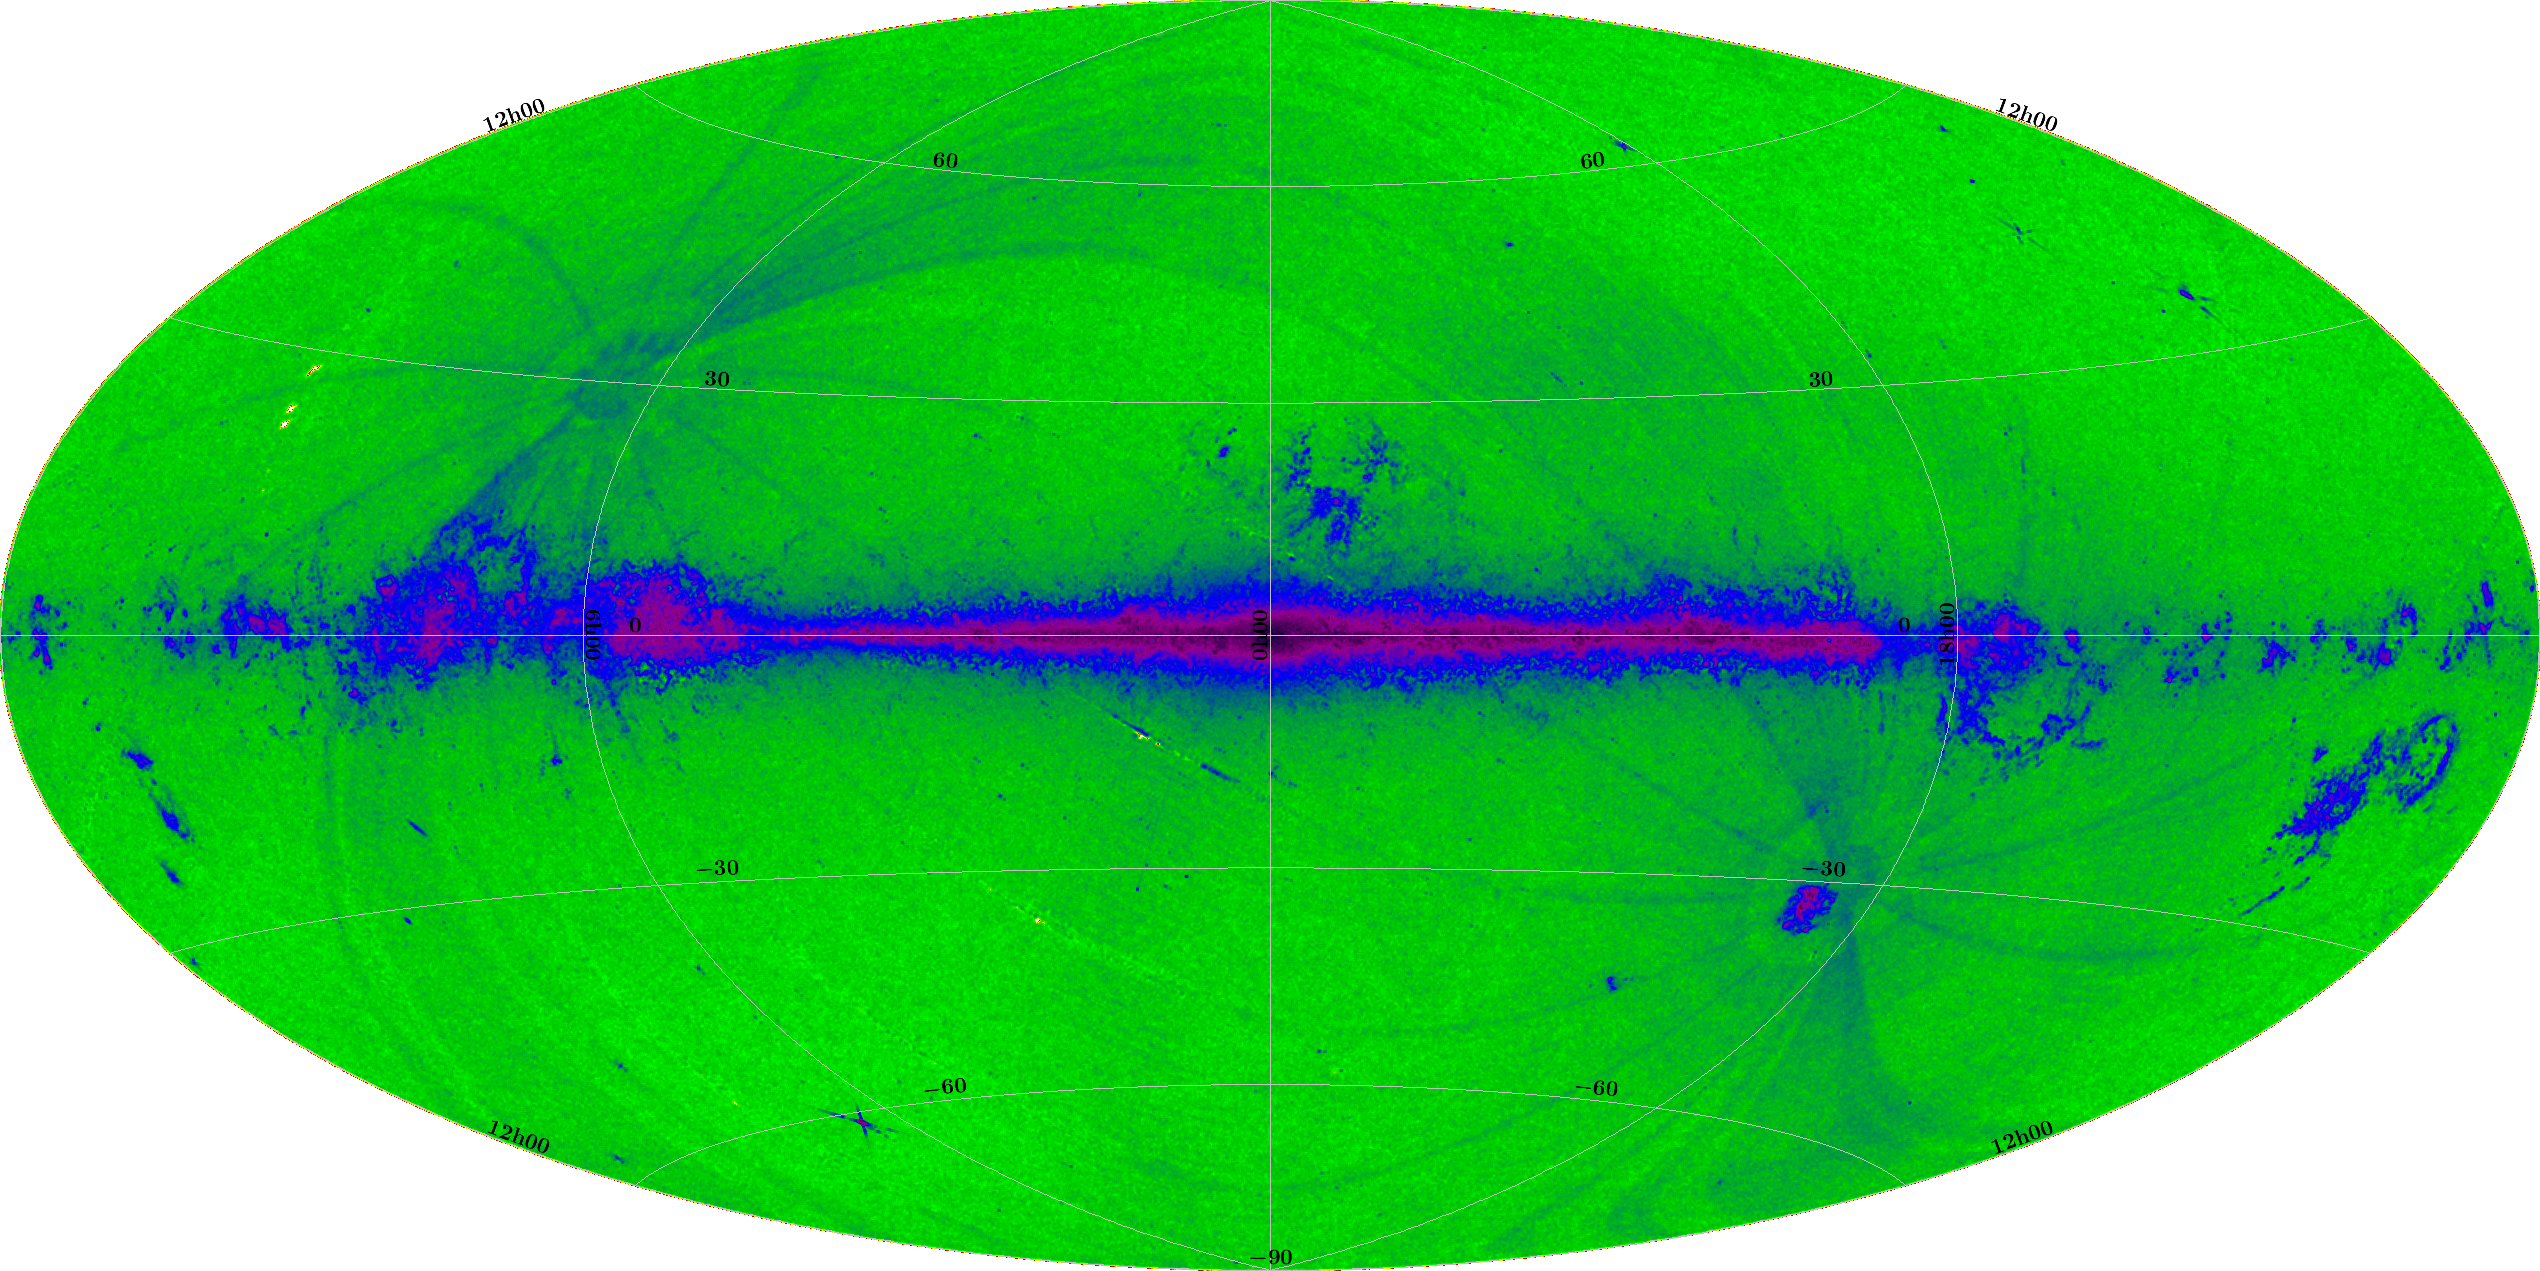
\includegraphics[height=10.0cm,width=16.0cm]
    {../../Gaia/plots/WISE_W4_DetBitge8_Aittoff_Galactic.png}
    \caption[The all-sky distribution of the 40.9M objects in the AllWISE W4 catalog.]
    {The all-sky distribution of the 40.9M objects in the AllWISE W4 catalog.
    The WISE scanning pattern can clearly be seen.}
    \label{fig:fig1}
\end{figure*}


\begin{figure}
   \centering
  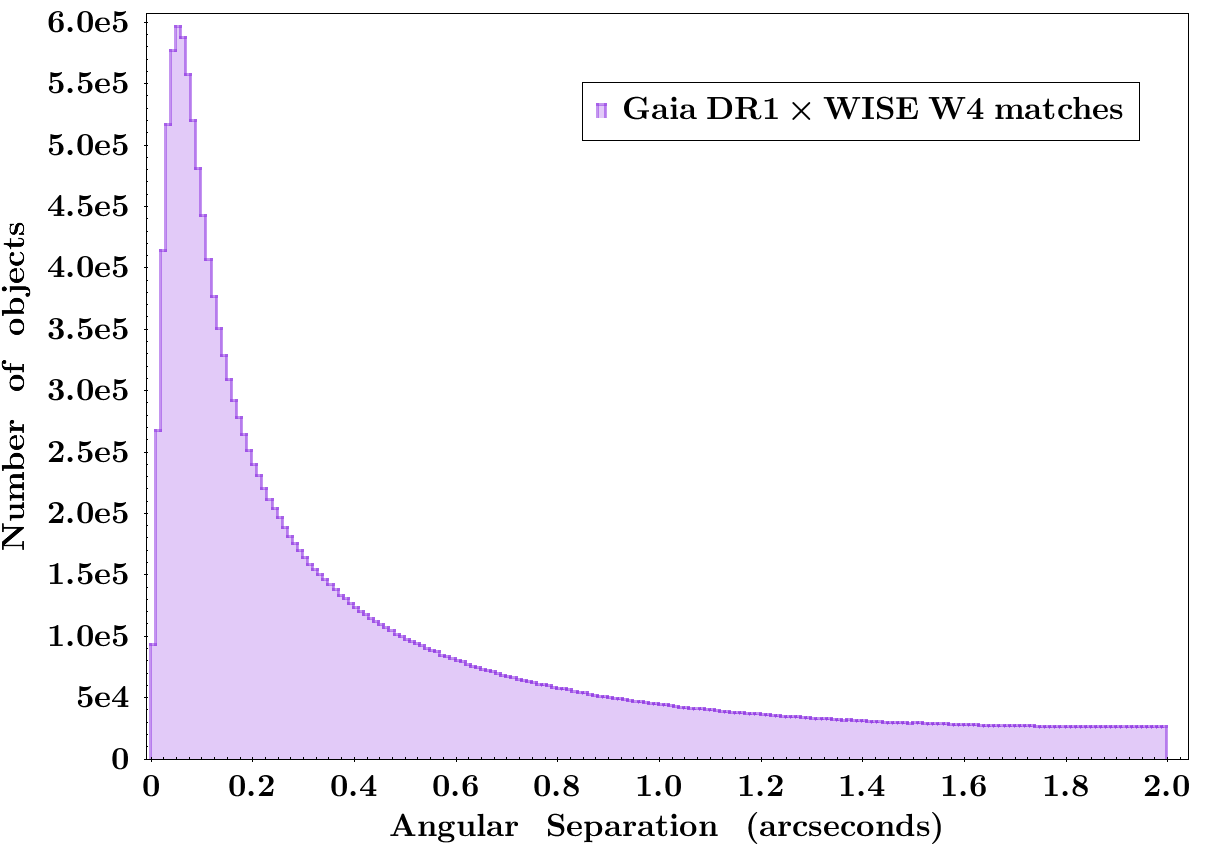
\includegraphics[height=8.0cm,width=8.0cm]
 {../../Gaia/plots/GaiaDR1xWISEW4_2as_histo.png}
    \caption[]
    {The matching radius separation histograms for objects, when a 2'' matching radius is applied.}
    \label{fig:fig2}
\end{figure}

\begin{figure}
    \centering
    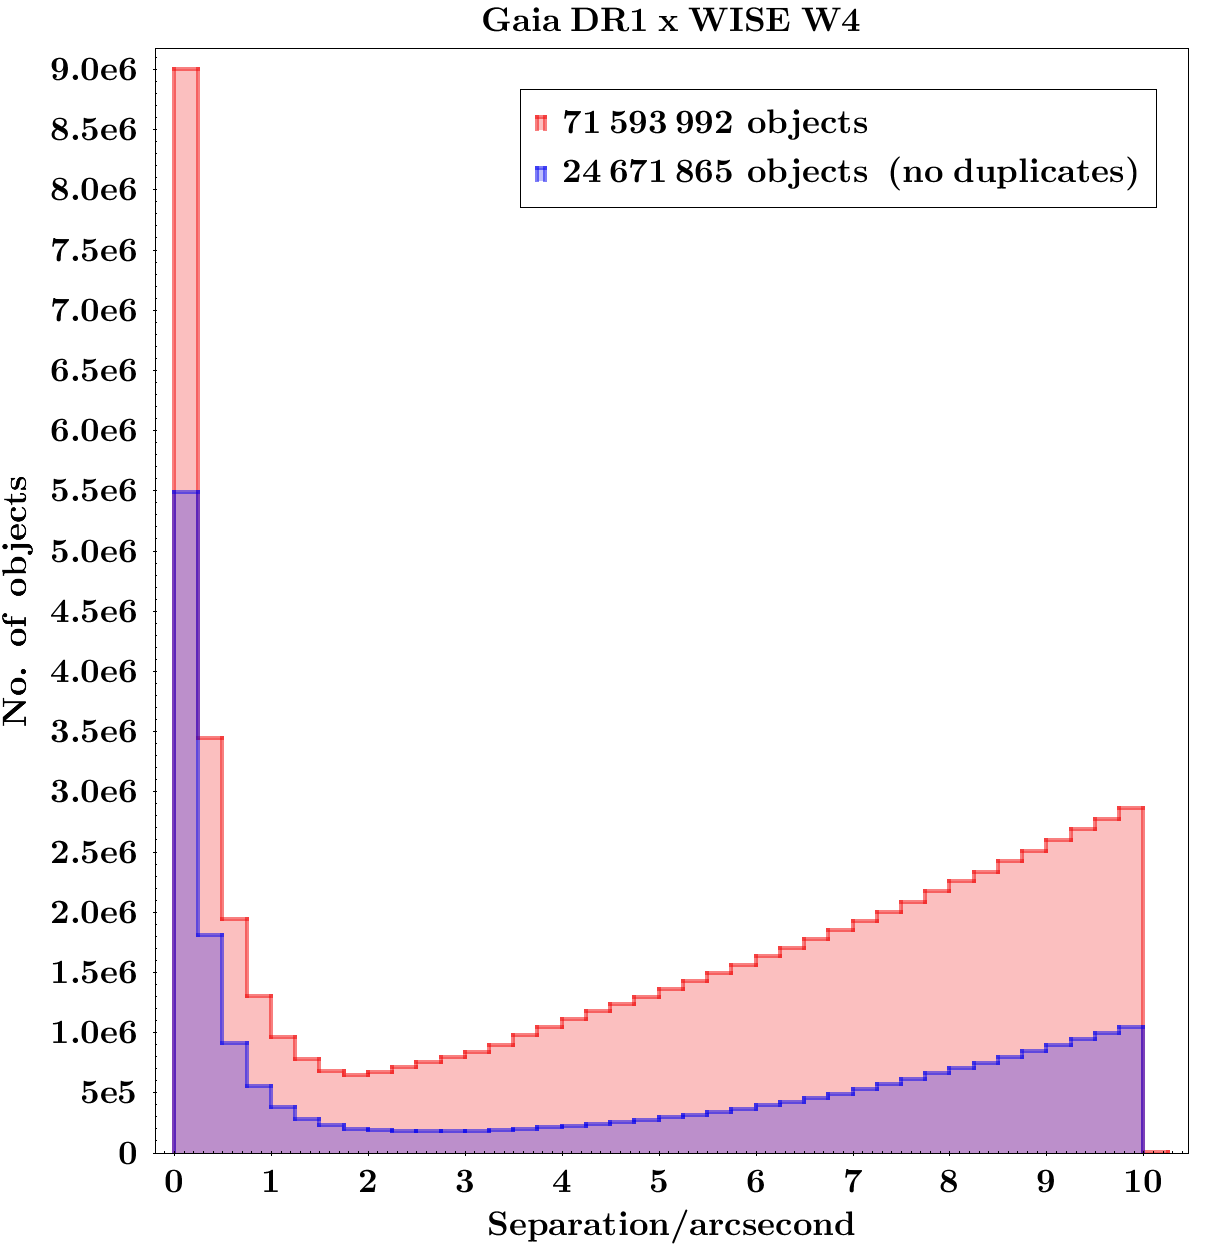
\includegraphics[height=8.0cm,width=8.0cm]
    {../../Gaia/plots/GaiaDR1xWISEW4_10asDupes_histo.png}
    \caption[The matching radius separation histograms for objects, with and without duplicates.]
    {The matching radius separation histograms for objects, when a 10'' matching radius is applied, with and without duplicates.}
    \label{fig:fig3}
\end{figure}

\begin{figure}
    \centering
    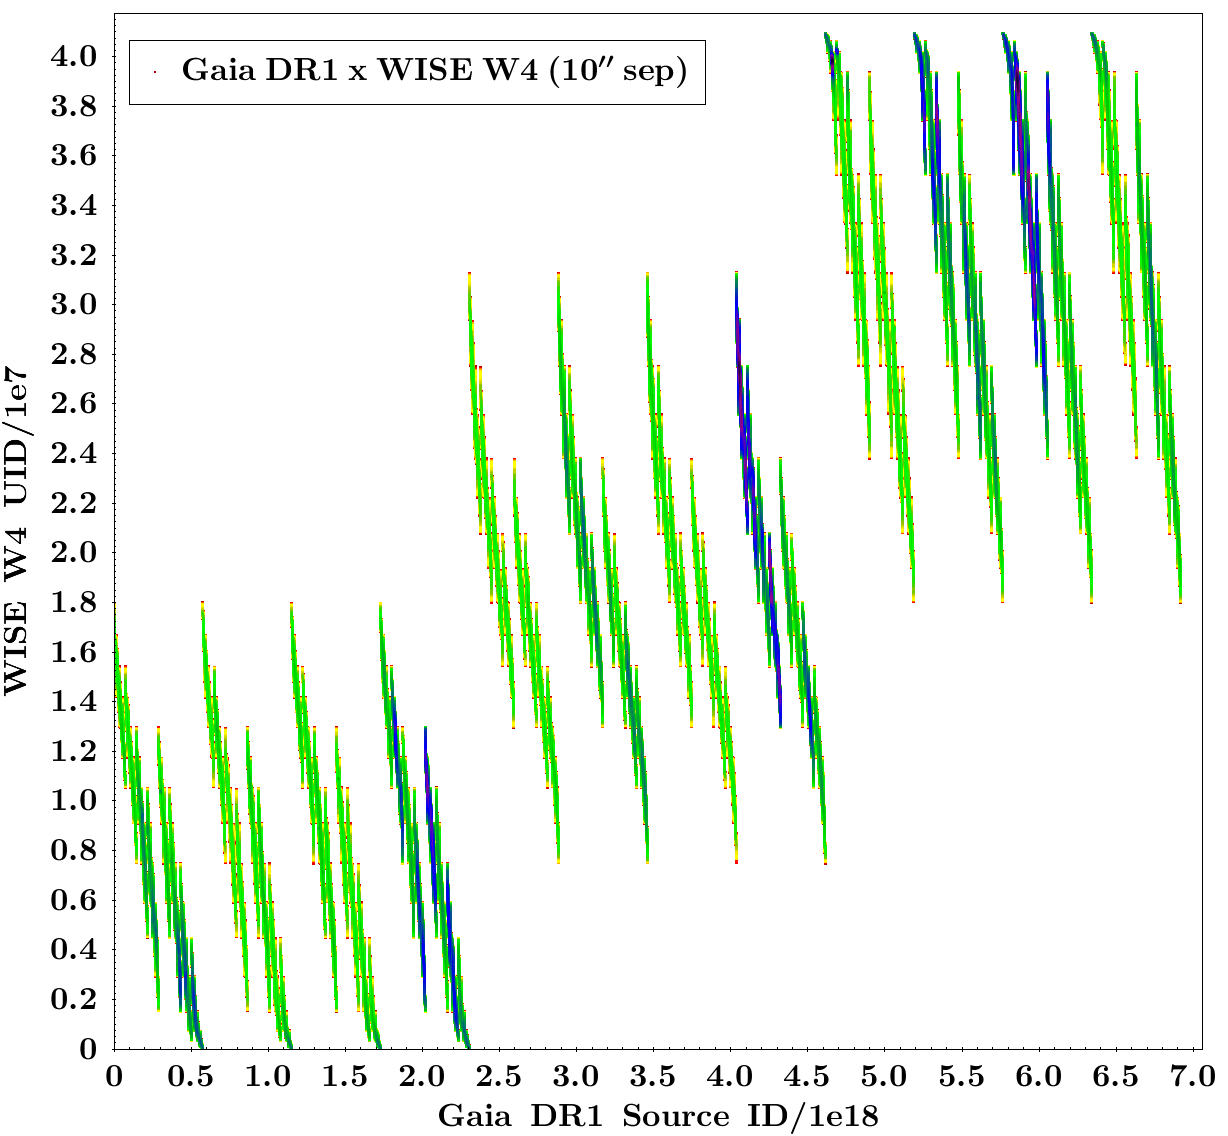
\includegraphics[height=8.0cm,width=8.0cm]
    {../../Gaia/plots/Gaia_sourceID_vs_WW4C_uid.png}
    \caption[The WISE W4 Unique ID (UID; which isa a proxy for object declination) versus the Gaia DR1 Source ID.]
    {The WISE W4 Unique ID (UID; which isa a proxy for object declination) versus the Gaia DR1 Source ID.}                    
    \label{fig:fig4}
\end{figure}



Figure~\ref{fig:fig5} (top) shows the all-sky distribution for the
full 40.9M objects that are detected in WISE W4 (same as
Figure~\ref{fig:fig1} but with a different
colour-scale). Figure~\ref{fig:fig5} (middle) shows the all-sky distrubtion of 
objects that were matched to a Gaia DR1 source. The overdensity of the Milky 
Way is clearly seen. Figure~\ref{fig:fig5} (bottom) shows the 16.3M objects 
that do {\it not} have a match in the Gaia DR1. 


\newpage
\centering
\begin{figure*}
\begin{center}
    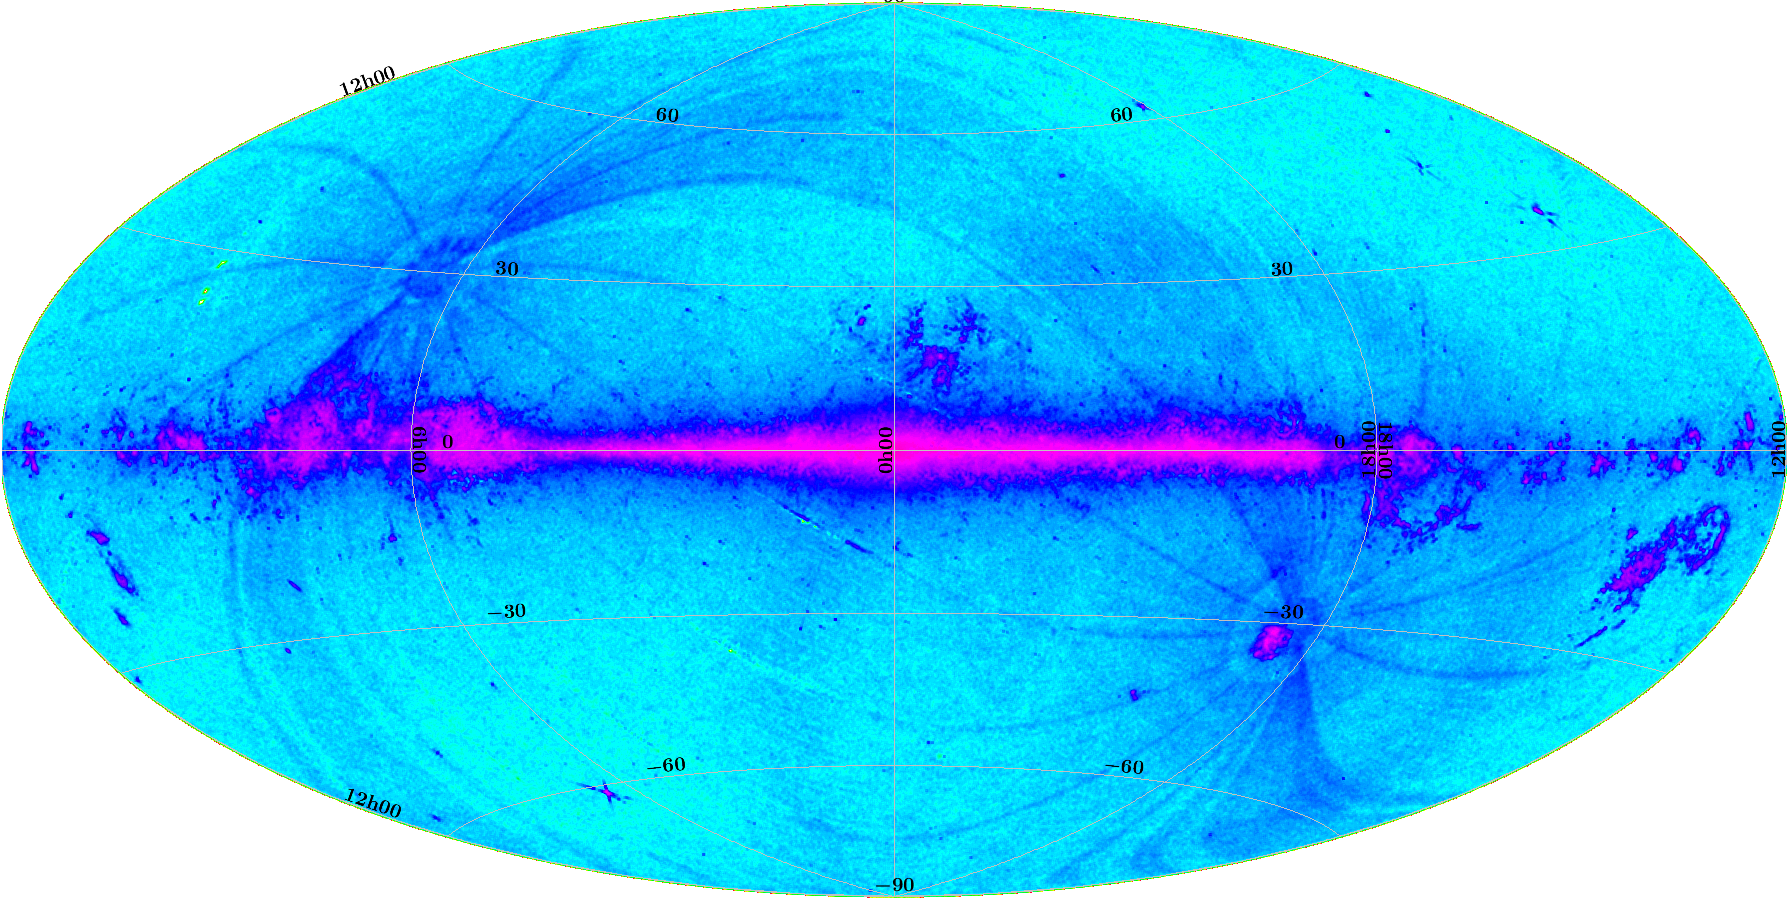
\includegraphics[height=7.5cm,width=14.0cm]{../../Gaia/plots/all_rainbow3.png}
    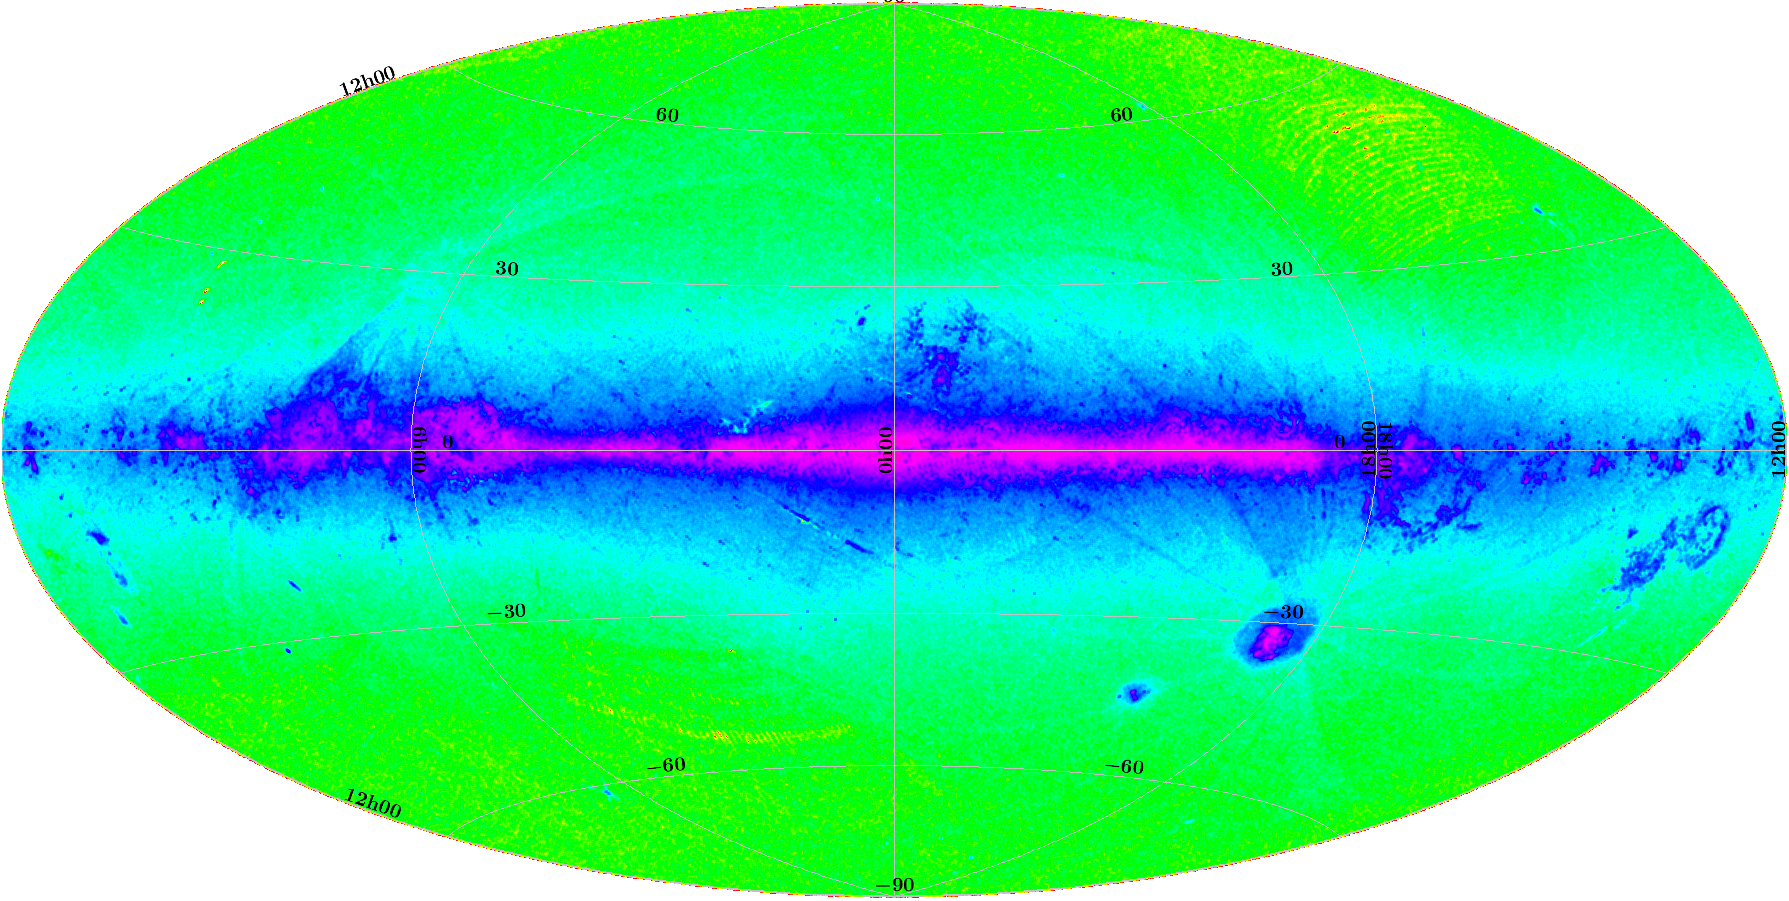
\includegraphics[height=7.5cm,width=14.0cm]{../../Gaia/plots/matches_rainbow3.png}
    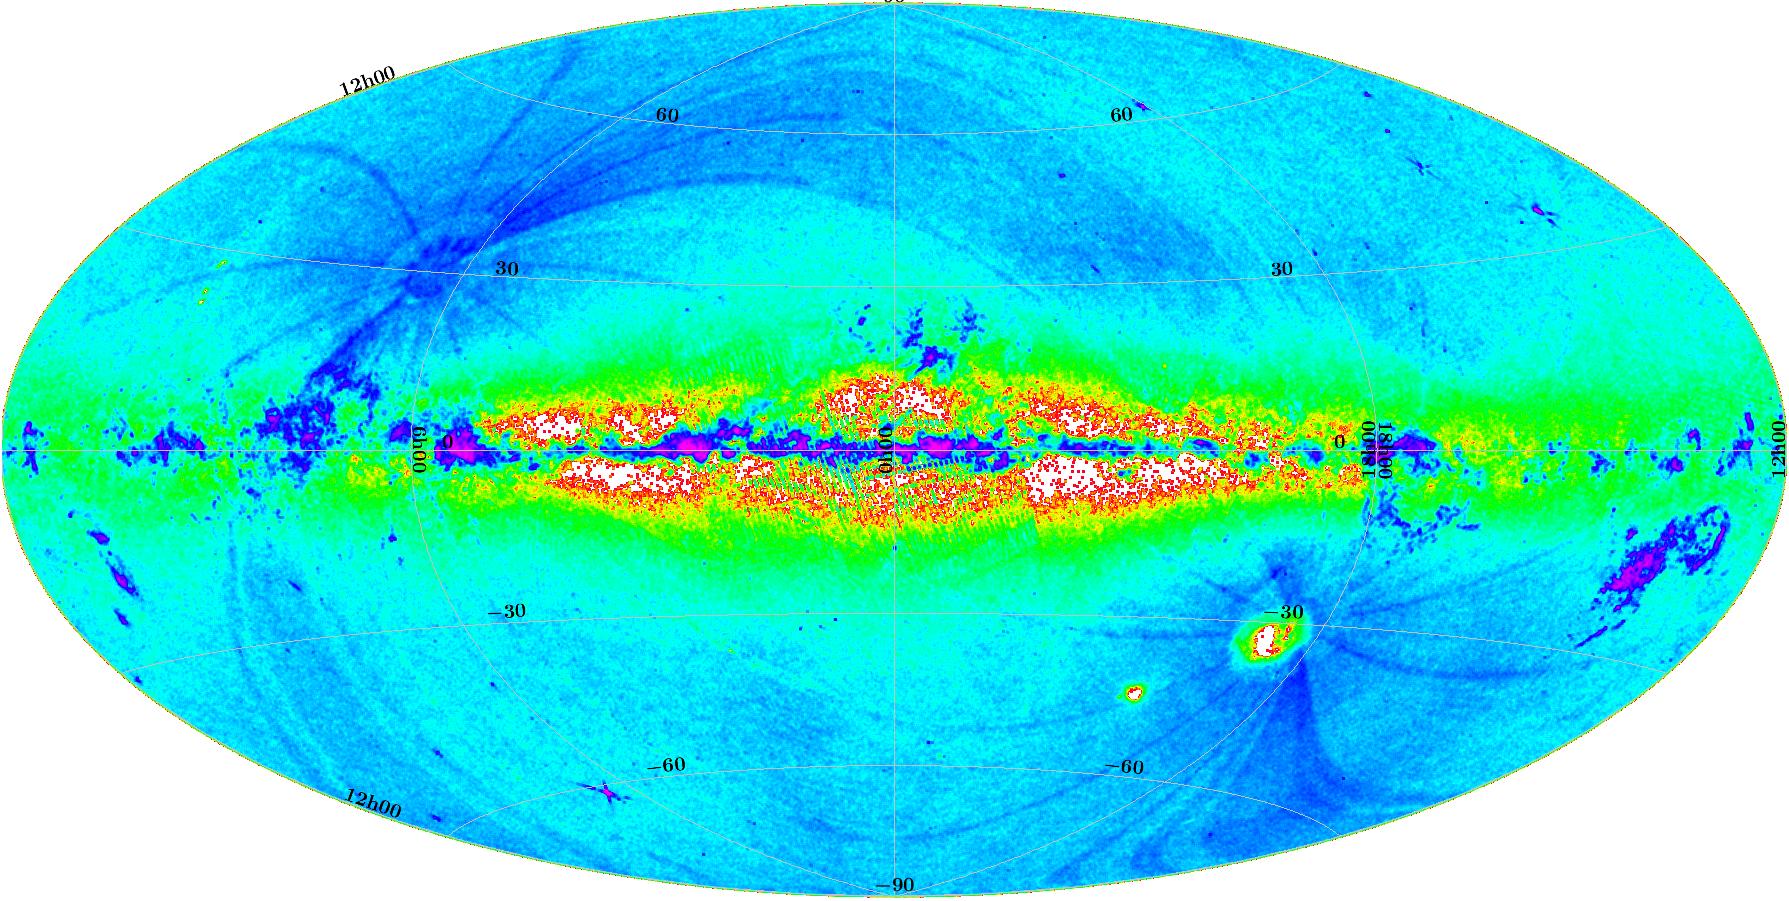
\includegraphics[height=7.5cm,width=14.0cm]{../../Gaia/plots/nonmatches_rainbow3.png}
    \caption[Lorem ipsum dolor sit amet, consectetur adipiscing elit. Aliquam porta sodales est, vel cursus risus porta non.]
    {Three aitoff projects for the Gaia DR1$\times$WISE W4 matched catalog.
    {\it Top:} The full 40.9M objects that are detected in WISE W4. 
    {\it Middle:}  The 24.7M WISE W4 objects that are matched to a Gaia DR1 source. 
    {\it Bottom:}  The 16.3M WISE W4 objects that are not matched to a Gaia DR1 source. 
  }
    \label{fig:fig5}
\end{center}
\end{figure*}






\bibliographystyle{mn2e}
\bibliography{/cos_pc19a_npr/LaTeX/tester_mnras}


\end{document}